\documentclass[11pt]{article}

\usepackage[utf8]{inputenc}
\usepackage[T1]{fontenc}
\usepackage{amsmath, amssymb, amsthm}
\usepackage{bm}
\usepackage{booktabs}
\usepackage{graphicx}
\usepackage{geometry}
\geometry{margin=1in}
\usepackage[numbers,sort&compress]{natbib}
\usepackage[colorlinks=true,linkcolor=blue,citecolor=blue,urlcolor=blue]{hyperref}

\theoremstyle{plain}
\newtheorem{theorem}{Theorem}
\newtheorem{lemma}{Lemma}
\newtheorem{corollary}{Corollary}
\theoremstyle{definition}
\newtheorem{definition}{Definition}
\theoremstyle{remark}
\newtheorem{remark}{Remark}

\DeclareMathOperator*{\argmin}{arg\,min}

% --- notation ---
\newcommand{\OPT}{\mathrm{OPT}}
\newcommand{\OPTLP}{\mathrm{OPT}_{\mathrm{LP}}}
\newcommand{\cost}{\mathrm{cost}}
\newcommand{\Ycal}{\mathcal{Y}}
\newcommand{\Pcal}{\mathcal{P}}
\newcommand{\Dcal}{\mathcal{D}}
\newcommand{\Ical}{\mathcal{I}}
\newcommand{\real}{\mathbb{R}}
\newcommand{\ratiohat}{\widehat{\mathrm{ratio}}}
\newcommand{\PDGNN}{\textsc{PD-GNN}}
\newcommand{\Greedy}{\textsc{Greedy}}
\newcommand{\LPRound}{\textsc{LP+Round}}
\newcommand{\GNNplain}{\textsc{GNN-plain}}

\title{\bfseries Primal--Dual Graph Networks: Aligning Message Passing with
Approximation Algorithms for Combinatorial Optimization on Graphs}
\author{Krishna Harish \\ Elkins High School}
\date{June 2026}

\begin{document}
\maketitle

\begin{abstract}
Graph neural networks (GNNs) are now a common tool for approximating solutions
to NP-hard combinatorial optimization (CO) problems. They have a basic
shortcoming: a network returns a candidate solution but says nothing about how
far that solution is from optimal. We address this with Primal--Dual Graph
Networks (\PDGNN), an architecture whose message passing is aligned with the
primal--dual schema used to design approximation algorithms. A \PDGNN{} carries
a primal state and a dual state at every node and edge and updates them over $T$
rounds that imitate the way a primal--dual algorithm raises dual variables and
rounds the primal. The network outputs an integral solution together with a
\emph{feasible} solution to the dual of the linear-programming (LP) relaxation.
Any feasible dual lower-bounds the optimum, so the ratio of the primal cost to
the dual value is an approximation \emph{certificate} that is valid for every
input, whatever the network has learned. We define primal--dual alignment,
prove that this certificate is always valid (Theorem~\ref{thm:cert}), and give a
generalization bound whose sample complexity is controlled by the number of
message-passing rounds and the maximum node degree rather than the number of
nodes. We then run the protocol on minimum-weight vertex cover over
Erd\H{o}s--R\'enyi and Barab\'asi--Albert graphs, with exact integer optima from
an ILP solver as ground truth. The learned dual head recovers a feasible dual
within a few percent of the LP optimum, so the self-certificate is tight and, as
guaranteed, always valid; we also report a negative finding---under the
size-normalized objective the primal scores collapse, so the integral cover is
produced by the repair layer rather than learned---which we trace to the
objective, not the architecture, and which leaves Theorem~\ref{thm:cert}
untouched. We close with the limitations of learned certificates and the main
open questions.
\end{abstract}

\section{Introduction}
Combinatorial optimization (CO) over graphs is central to theoretical computer
science. Vertex cover, set cover, maximum independent set, facility location,
and the traveling salesman problem are standard NP-hard problems, and the effort
to solve them approximately produced much of the modern theory of approximation
algorithms~\citep{williamson2011design}. Separately, a growing line of work uses
deep learning, and graph neural networks in particular, to learn heuristics for
these problems directly from data~\citep{khalil2017learning, bello2016neural,
gasse2019exact}. A learned model can specialize to the distribution of instances
a user actually sees, and on that distribution it sometimes beats a
general-purpose solver.

Learned CO models share one feature that limits their use: they behave as black
boxes. A GNN returns a candidate solution, but it does not tell you whether that
solution is within one percent or a factor of ten of optimal. Without this
information a user cannot separate a good answer from a bad one short of solving
the instance exactly, which is the work the model was supposed to save.
Classical approximation algorithms do not have this problem. The primal--dual
method, one of the most widely used design techniques in the
area~\citep{williamson2011design}, builds a feasible dual solution alongside
every integral solution. Weak LP duality makes that dual a certified bound on
the optimum, so the algorithm returns an answer \emph{and} a proof of how good
the answer is.

We ask whether a neural network can keep this guarantee by construction. The
starting point is that the architecture, not just the loss, should reflect the
algorithm we want to imitate. This is the algorithmic alignment idea of
\citet{xu2020what} and the neural algorithmic reasoning program of
\citet{velivckovic2021neural}: when a network's computation graph matches the
data flow of a target algorithm, it needs fewer samples to learn the algorithm
and generalizes more reliably. We apply this idea to the primal--dual schema.

\paragraph{Contributions.}
\begin{enumerate}
\item \textbf{Architecture (Section~\ref{sec:arch}).} \PDGNN{} is a
message-passing network that carries coupled primal and dual states. Each round
follows one step of a primal--dual approximation algorithm, and the network ends
in a primal rounding layer and a dual feasibility projection. It outputs an
integral solution and a feasible dual.
\item \textbf{Always-valid certificates (Section~\ref{sec:theory},
Theorem~\ref{thm:cert}).} The dual head is constrained to the dual-feasible
region, so the reported ratio of primal cost to dual value upper-bounds the
realized approximation ratio for every input and every choice of parameters.
This holds whether or not training succeeded. We regard this as the paper's
central and cleanest result.
\item \textbf{Alignment and generalization (Section~\ref{sec:theory},
Theorem~\ref{thm:gen}).} We define primal--dual alignment and prove a
uniform-convergence bound whose sample complexity depends on the number of
message-passing rounds $T$ and the Lipschitz constants of the update modules,
not on the number of nodes $n$ directly.
\end{enumerate}
Section~\ref{sec:exp} gives the protocol and real results, and
Section~\ref{sec:conc} discusses limitations.

\section{Related Work}\label{sec:rel}

\paragraph{Learning for combinatorial optimization.}
Pointer networks~\citep{vinyals2015pointer} and later reinforcement-learning
formulations~\citep{bello2016neural} learn to construct solutions to routing
problems. \citet{khalil2017learning} pair a graph embedding with $Q$-learning to
build solutions to graph problems greedily. \citet{gasse2019exact} learn
branching rules for branch-and-bound with a bipartite-graph GNN. These methods
aim at solution quality and give no instance-specific bound, so our goal of
producing the certificate is complementary to theirs.

\paragraph{Duality in neural algorithmic reasoning.}
Two lines are closest to us, and both bring duality into neural algorithmic
reasoning, but for a different purpose. \citet{numeroso2023dual} exploit the
max-flow/min-cut theorem to co-learn a primal algorithm (max-flow) and its dual
(min-cut) on the CLRS benchmark; duality is an \emph{auxiliary training signal}
that improves representation learning and generalization. The learned cut is an
ordinary network output with no feasibility guarantee, and the method reports no
duality-gap bound; it also targets a strong-duality, polynomial-time problem,
where a one-sided certificate is not the point. \citet{he2025primal} align a GNN
with the primal--dual schema through a bipartite primal--dual graph (a primal
variable per vertex, a dual variable per edge, a packing constraint per vertex)
and target NP-hard covering problems including vertex cover and set cover. Their
headline contribution is to add \emph{optimal} solutions on small instances as
supervision so the network \emph{outperforms} the approximation algorithm it
imitates; their guarantee is therefore \emph{a-priori}---the architecture can
exactly replicate the classical algorithm and so inherits its worst-case
ratio---an expressivity statement about what the architecture can represent,
not a per-instance bound on what the trained network actually output.

Unlike both, \PDGNN{} constrains the dual head to the LP-feasible region
\emph{by construction} (a feasibility projection in the forward pass) and reports
cost/dual as an \emph{a-posteriori}, instance-specific certificate that is valid
for every input regardless of whether training succeeded. In one line: prior
primal--dual reasoning uses duality to \emph{learn better solutions}; we use a
feasible dual to \emph{certify} the solution we produce, turning weak LP duality
into an instance-specific guarantee that survives a failed run.\footnote{The
name \PDGNN{} is close to the ``Primal--Dual Graph Neural Networks (PDGNN)'' of
\citet{he2025primal}. The two are distinct: their contribution is alignment plus
optimal supervision to beat the algorithm with an a-priori guarantee; ours is an
architectural feasibility projection that yields an always-valid a-posteriori
certificate. We retain the abbreviation but flag the overlap to avoid confusion.}

\paragraph{Graph neural networks and alignment.}
Our architecture is a message-passing network~\citep{gilmer2017neural} in the
line of \citet{kipf2017semi}, specialized so that the message and update
functions carry two interacting channels. The expressive power of message
passing is limited by the Weisfeiler--Leman hierarchy, which restricts what any
such model can compute; we treat this as a design constraint and return to it in
Section~\ref{sec:conc}. \citet{xu2020what} show that aligning a network with a
target algorithm improves sample complexity, and \citet{velivckovic2021neural}
set out the broader aim of running classical algorithms inside neural networks.
We take this in a specific direction: toward primal--dual approximation
algorithms and toward one guarantee, a valid duality certificate. The
primal--dual method gives a $2$-approximation for weighted vertex cover, an
$O(\log n)$-approximation for set cover, and constant-factor approximations for
several network-design problems~\citep{williamson2011design}; we use it both as
the inductive bias for the architecture and as the source of the certificate.

\section{Mathematical Formulation}\label{sec:form}

\subsection{Problem class}
We study weighted covering problems on graphs and use minimum-weight vertex
cover as the running example. The formulation carries over to weighted set cover
once the vertex--edge incidence is replaced by a general set--element incidence.

Let $G=(V,E)$ be an undirected graph with $n=|V|$ nodes and nonnegative node
weights $w\in\real_{\ge 0}^V$. A vertex cover is a set $S\subseteq V$ that meets
every edge. The integer program (IP) and its LP relaxation are
\begin{align}
\OPT(G,w) &= \min_{x\in\{0,1\}^V} \sum_{v\in V} w_v x_v
   \quad\text{s.t.}\quad x_u+x_v\ge 1 \ \ \forall (u,v)\in E, \label{eq:ip}\\
\OPTLP(G,w) &= \min_{x\in[0,1]^V} \sum_{v\in V} w_v x_v
   \quad\text{s.t.}\quad x_u+x_v\ge 1 \ \ \forall (u,v)\in E. \label{eq:lp}
\end{align}
The dual of \eqref{eq:lp} puts a variable $y_e\ge 0$ on each edge:
\begin{equation}
\max_{y\in\real_{\ge0}^E} \sum_{e\in E} y_e
   \quad\text{s.t.}\quad \sum_{e\ni v} y_e \le w_v \ \ \forall v\in V. \label{eq:dual}
\end{equation}
Write $\Pcal=[0,1]^V$ for the primal box and
$\Ycal(G,w)=\bigl\{\,y\in\real_{\ge0}^E : \sum_{e\ni v} y_e\le w_v\ \forall v\in V\,\bigr\}$
for the dual feasible region. Weak duality gives the chain that motivates the
rest of the paper:
\begin{equation}
\sum_{e\in E} y_e \ \le\ \OPTLP(G,w) \ \le\ \OPT(G,w)
   \qquad\text{for all } y\in\Ycal(G,w). \label{eq:weak}
\end{equation}

\subsection{The primal--dual template}
The standard primal--dual $2$-approximation keeps a feasible dual $y$ and a
primal set $S$. It picks a violated edge, raises that edge's dual variable until
some node constraint $\sum_{e\ni v} y_e=w_v$ becomes tight, and adds every newly
tight node to $S$, stopping once $S$ is feasible. The returned $S$ satisfies
$\cost(S)\le 2\sum_e y_e\le 2\,\OPT$. We abstract this as a map
\begin{equation}
\Phi:(G,w)\longmapsto (S,y),\qquad S\text{ feasible for \eqref{eq:ip}},\ \ y\in\Ycal(G,w),\label{eq:phi}
\end{equation}
realized by $T$ rounds of a local update. We take $\Phi$ to be a
\emph{synchronous, bounded-round} version of the schema that proposes dual
increments on all edges in parallel each round and then restores feasibility, so
$T$ is a small design parameter rather than the (typically large) number of
single-edge updates the classical sequential algorithm performs. \PDGNN{} is a
learnable surrogate for this $\Phi$ in which the per-round update is a neural
module, while the feasibility structure---$y\in\Ycal$ and $S$ a cover---is
enforced exactly by projection and rounding layers.

\subsection{Notation for the learned model}
A \PDGNN{} with parameters $\theta$ computes a function
\[
f_\theta:(G,w)\longmapsto (\hat x,\hat y)\in[0,1]^V\times\Ycal(G,w),
\]
from which an integral cover $\hat S=\rho(\hat x,G)$ is obtained by the rounding
map $\rho$ of Section~\ref{sec:arch}. We write $h_v^{(t)}\in\real^d$ and
$g_e^{(t)}\in\real^d$ for the primal node state and dual edge state at round $t$,
and reserve $\mu_v^{(t)},\nu_e^{(t)}\in\real$ for the scalar read-outs that
become $\hat x_v$ and $\hat y_e$.

\section{Proposed Architecture: PD-GNN}\label{sec:arch}
\PDGNN{} has an encoder, $T$ rounds of primal--dual message passing, and two
output heads with feasibility layers.

\subsection{Encoder}
Each node gets an initial primal state from its weight and degree, and each edge
a dual state initialized at zero dual mass,
\[
h_v^{(0)}=\phi_{\mathrm{enc}}\bigl([\,w_v,\ \deg(v)\,]\bigr),\qquad
g_e^{(0)}=\psi_{\mathrm{enc}}\bigl([\,w_u,w_v\,]\bigr),\qquad \nu_e^{(0)}=0,\ \ e=(u,v),
\]
where $\phi_{\mathrm{enc}}$ and $\psi_{\mathrm{enc}}$ are multilayer perceptrons
(MLPs).

\subsection{Primal--dual message passing}
At round $t=0,\dots,T-1$ we run a dual ascent step and then a coupled primal
step. These follow the ``raise a dual variable'' and ``add tight vertices''
moves of the template $\Phi$.

\emph{(i) Dual update.} For each edge $e=(u,v)$ the model proposes a nonnegative
increment $\delta_e^{(t)}\ge 0$ from the local states of its endpoints:
\begin{equation}
\delta_e^{(t)}=\mathrm{ReLU}\!\bigl(m_{\mathrm{dual}}(g_e^{(t)},h_u^{(t)},h_v^{(t)})\bigr),
\qquad \tilde\nu_e^{(t+1)}=\nu_e^{(t)}+\delta_e^{(t)}, \label{eq:dualinc}
\end{equation}
with $m_{\mathrm{dual}}$ an MLP. The raw increments need not respect the node
constraints, so we apply a dual feasibility projection $\Pi_\Ycal$
(Section~\ref{sec:heads}) that returns $\nu^{(t+1)}=\Pi_\Ycal(\tilde\nu^{(t+1)})
\in\Ycal(G,w)$. The edge state is then refreshed:
$g_e^{(t+1)}=u_{\mathrm{dual}}(g_e^{(t)},\nu_e^{(t+1)},h_u^{(t)},h_v^{(t)})$.

\emph{(ii) Primal update with complementary-slackness coupling.} Each node
aggregates the dual mass currently incident to it, $s_v^{(t+1)}=\sum_{e\ni v}
\nu_e^{(t+1)}$, and computes a slack $\sigma_v^{(t+1)}=w_v-s_v^{(t+1)}\ge 0$,
where nonnegativity is guaranteed by the projection. Complementary slackness says
a node should enter the cover roughly when its slack vanishes, so we let the
model learn a smooth version of this rule:
\begin{equation}
h_v^{(t+1)}=u_{\mathrm{prim}}\Bigl(h_v^{(t)},\ \sigma_v^{(t+1)},\
   \textstyle\sum_{u\sim v} m_{\mathrm{prim}}(h_u^{(t)},\nu_{(u,v)}^{(t+1)})\Bigr),
\qquad \mu_v^{(t+1)}=\mathrm{sigmoid}\bigl(a^\top h_v^{(t+1)}+b\bigr). \label{eq:prim}
\end{equation}
The vector $a$ and scalar $b$ are shared readout parameters. The explicit slack
input $\sigma_v$ is the device that aligns the primal channel with the dual
channel: a node's tendency to be selected is wired to its dual tightness instead
of being left for the model to discover.

\subsection{Output heads and feasibility layers}\label{sec:heads}
\emph{Dual feasibility projection $\Pi_\Ycal$.} Given raw edge masses
$\tilde\nu\ge 0$, define the per-node load $\ell_v=\sum_{e\ni v}\tilde\nu_e$ and
the per-node admissible scale $\lambda_v=\min\{1,\,w_v/\ell_v\}$, with
$\lambda_v=1$ when $\ell_v=0$. Setting
\begin{equation}
\nu_e=\Bigl(\min_{v\in e}\lambda_v\Bigr)\tilde\nu_e \label{eq:proj}
\end{equation}
gives $\nu\in\Ycal(G,w)$, since for every node $v$ we have
$\sum_{e\ni v}\nu_e\le\lambda_v\ell_v\le w_v$. The map \eqref{eq:proj} is
continuous and piecewise differentiable, so it admits backpropagation.

\emph{Primal rounding $\rho$.} From the final primal scores $\mu_v^{(T)}$ we
obtain an integral cover by thresholding and a repair pass: set
$\hat x_v=\mathbf{1}[\mu_v^{(T)}\ge\frac12]$, then, while any edge $(u,v)$ is
uncovered, add its cheaper endpoint, $\hat x_{\argmin_{z\in\{u,v\}} w_z}\!\gets1$.
The repair pass guarantees that $\hat S=\{v:\hat x_v=1\}$ is always a feasible
cover.

\emph{Outputs.} The model returns the cover $\hat S$ with cost
$\cost(\hat S)=\sum_{v\in\hat S} w_v$, the dual $\hat y=\nu^{(T)}\in\Ycal$ with
value $D(\hat y)=\sum_e\hat y_e$, and the self-reported certificate
\begin{equation}
\ratiohat=\frac{\cost(\hat S)}{D(\hat y)}\qquad(\text{set to }+\infty\text{ if } D(\hat y)=0). \label{eq:ratio}
\end{equation}

\begin{figure}[t]
\centering
\fbox{\begin{minipage}{0.92\linewidth}
\textbf{Algorithm 1: \PDGNN{} forward pass}\\[2pt]
\textbf{input:} graph $G=(V,E)$, weights $w$; rounds $T$; parameters $\theta$.
\begin{enumerate}\setlength{\itemsep}{1pt}
\item initialize $h_v^{(0)},g_e^{(0)},\nu_e^{(0)}=0$ via encoders.
\item \textbf{for} $t=0$ \textbf{to} $T-1$:
  \begin{itemize}\setlength{\itemsep}{0pt}
  \item[2a.] propose dual increments $\delta_e^{(t)}\ge 0$ \hfill (Eq.~\ref{eq:dualinc})
  \item[2b.] project $\nu^{(t+1)}\gets\Pi_\Ycal(\nu^{(t)}+\delta^{(t)})$ \hfill (Eq.~\ref{eq:proj})
  \item[2c.] compute slacks $\sigma_v^{(t+1)}=w_v-\sum_{e\ni v}\nu_e^{(t+1)}$
  \item[2d.] update primal states $h_v^{(t+1)},\mu_v^{(t+1)}$ \hfill (Eq.~\ref{eq:prim})
  \end{itemize}
\item round $\hat S\gets\rho(\mu^{(T)},G)$; set $\hat y\gets\nu^{(T)}$.
\item \textbf{return} $\hat S$, $\hat y$, and $\ratiohat=\cost(\hat S)/D(\hat y)$.
\end{enumerate}
\end{minipage}}
\caption{The forward pass alternates a feasibility-projected dual step (2a, 2b)
with a slack-coupled primal update (2c, 2d), then rounds and computes the
certificate.}
\label{fig:alg}
\end{figure}

\subsection{Training objective}
Given a distribution $\Dcal$ over instances $(G,w)$, we train $\theta$ to make
the cover cheap and keep the dual large, which keeps the certificate tight. With
a hyperparameter $\beta>0$ the per-instance loss is the size-normalized objective
\begin{equation}
\mathcal{L}_\theta(G,w)=\frac1n\underbrace{\sum_v w_v\,\mu_v^{(T)}}_{\text{soft primal cost}}
   -\ \frac{\beta}{n}\underbrace{\sum_e \hat y_e}_{\text{dual value}}. \label{eq:loss}
\end{equation}
The $1/n$ normalization keeps the loss in a bounded range that does not grow with
graph size, which we rely on in the generalization analysis of
Section~\ref{sec:theory}. Both terms are differentiable in $\theta$: the dual
term through the projection \eqref{eq:proj}, and the primal term through the soft
scores $\mu_v^{(T)}$. The integral rounding $\rho$ is used only at evaluation, so
no discrete-gradient estimator is needed. Feasibility of $\hat y$ and $\hat S$
comes from the architecture, not the loss; the loss only controls quality. We
return in Section~\ref{sec:exp} to a consequence of \eqref{eq:loss} we did not
anticipate: it places no reward on the primal scores being large anywhere, so
the soft scores collapse and the cover is determined by the repair pass.

\section{Theoretical Analysis}\label{sec:theory}
We first record the safety property and then the generalization result.
Throughout, $\|\cdot\|$ is the Euclidean norm and all MLPs use $1$-Lipschitz
activations such as ReLU.

\subsection{The certificate is always valid}
\begin{theorem}[Validity of the self-certificate]\label{thm:cert}
For every graph $G$, every weight vector $w\in\real_{\ge0}^V$, and every
parameter setting $\theta$, the \PDGNN{} outputs a feasible cover $\hat S$ and a
dual-feasible $\hat y\in\Ycal(G,w)$ with
\[
D(\hat y)\ \le\ \OPT(G,w)\ \le\ \cost(\hat S),
\qquad\text{so}\qquad
1\ \le\ \frac{\cost(\hat S)}{\OPT(G,w)}\ \le\ \ratiohat=\frac{\cost(\hat S)}{D(\hat y)}.
\]
The reported number $\ratiohat$ is therefore always a valid upper bound on the
true approximation ratio achieved on that instance, regardless of training.
\end{theorem}
\begin{proof}
Feasibility of $\hat y$ follows from the projection: by \eqref{eq:proj},
$\sum_{e\ni v}\hat y_e\le w_v$ for all $v$ and $\hat y\ge 0$, so
$\hat y\in\Ycal(G,w)$. Feasibility of $\hat S$ follows from the repair pass in
$\rho$, which stops only when no edge is uncovered. Weak duality \eqref{eq:weak}
gives $D(\hat y)=\sum_e\hat y_e\le\OPT(G,w)$, while $\hat S$ feasible gives
$\OPT(G,w)\le\cost(\hat S)$. Dividing by $\OPT$, which is positive whenever
$E\neq\emptyset$ and some incident weight is positive and otherwise makes the
claim trivial, yields the displayed chain.
\end{proof}

\begin{remark}\label{rem:honest}
This is what alignment buys in practice: a heuristic that reports an
\emph{honest}, instance-specific bound. A poorly trained network gives a loose
certificate, meaning a large $\ratiohat$; it cannot give a false one. Black-box
CO learners do not have this property. We stress that Theorem~\ref{thm:cert} does
\emph{not} say \PDGNN{} inherits the worst-case $2$-approximation of the
template, because the learned modules can output any feasible pair. The only
guarantee on solution quality is the a-posteriori certificate, whose value
depends on training. This separation---a worst-case-free architecture with an
always-valid bound---is exactly the property we verify empirically in
Section~\ref{sec:exp}.
\end{remark}

\subsection{Primal--dual alignment and sample complexity}
We now say what it means for the architecture to be aligned with the template
$\Phi$, and show that alignment gives a generalization bound that does not depend
on $n$ directly. Let $\Delta$ bound the maximum degree and $W$ bound the node
weights, so instances lie in a class $\Ical_{\Delta,W}$.

\begin{definition}[$(T,L)$ primal--dual alignment]\label{def:align}
A \PDGNN{} is $(T,L)$-\emph{aligned} with the primal--dual template if (i) it
uses exactly $T$ rounds, matching the $T$ rounds of the bounded-round scheme
$\Phi$, (ii) each learnable module $m_{\mathrm{dual}},u_{\mathrm{dual}},
m_{\mathrm{prim}},u_{\mathrm{prim}}$ is $L$-Lipschitz in its inputs, and (iii)
the feasibility maps $\Pi_\Ycal$ and $\rho$ are exactly the structural operations
of $\Phi$, namely projection to $\Ycal$ and cover rounding, shared rather than
learned.
\end{definition}

\begin{lemma}[State stability]\label{lem:stab}
Under $(T,L)$-alignment with $L$-Lipschitz, $B$-bounded modules and degree bound
$\Delta$, the map from parameters to the final node scores and edge duals is
Lipschitz: there is a constant $\kappa(T,L,\Delta)\le C\,(L\Delta)^T$ for an
absolute constant $C$, such that for parameter vectors $\theta,\theta'$,
\[
\bigl\|\mu^{(T)}(\theta)-\mu^{(T)}(\theta')\bigr\|_\infty\le\kappa\,\|\theta-\theta'\|
\quad\text{and}\quad
\bigl\|\nu^{(T)}(\theta)-\nu^{(T)}(\theta')\bigr\|_\infty\le\kappa\,\|\theta-\theta'\|.
\]
\end{lemma}
\begin{proof}[Proof sketch]
Each round composes (a) the $L$-Lipschitz modules, (b) a sum of at most $\Delta$
incident messages, which scales the Lipschitz constant by at most $\Delta$, and
(c) the projection $\Pi_\Ycal$, which contributes a constant Lipschitz factor
because it multiplies its inputs by scalars $\min_{v\in e}\lambda_v\in[0,1]$ that
vary in a bounded, piecewise-smooth way with the loads. Composing $T$ such rounds
multiplies the per-round constant $O(L\Delta)$, giving $\kappa=O((L\Delta)^T)$.
The final sigmoid readout is $1$-Lipschitz, and boundedness keeps the constants
finite.
\end{proof}

\begin{theorem}[Generalization under alignment]\label{thm:gen}
Fix a $(T,L)$-aligned \PDGNN{} with parameters in a Euclidean ball of radius $R$
and $P$ coordinates, weights bounded by $W$, and degree bounded by $\Delta$. The
size-normalized loss \eqref{eq:loss} takes values in an interval of width
$M=O(1+\beta\Delta)$. For a sample of $N$ i.i.d.\ instances from $\Dcal$, with
probability at least $1-\delta$, every parameter $\theta$ in the ball satisfies
\[
\mathbb{E}_{(G,w)\sim\Dcal}[\mathcal{L}_\theta]\ \le\
\frac1N\sum_{i=1}^N\mathcal{L}_\theta(G_i,w_i)\ +\
c\,M\sqrt{\frac{P\log\bigl(1+\kappa(T,L,\Delta)\,R\,N\bigr)+\log(1/\delta)}{N}},
\]
for an absolute constant $c$, where $\kappa(T,L,\Delta)=O((L\Delta)^T)$ is the
Lipschitz constant of Lemma~\ref{lem:stab}.
\end{theorem}
\begin{proof}[Proof sketch]
By Lemma~\ref{lem:stab} and the $1/n$ normalization in \eqref{eq:loss}, the loss
is $O((W+\beta\Delta)\kappa)$-Lipschitz in $\theta$: the per-node average
$\frac1n\sum_v w_v\mu_v$ has Lipschitz constant at most $W\kappa$ because the
$1/n$ cancels the $n$ summed node terms, and the dual average contributes at most
$O(\beta\Delta\kappa)$ since a bounded-degree graph has $O(n\Delta)$ edges. An
$\epsilon$-net of the radius-$R$ ball in $\real^P$ induces an
$O((W+\beta\Delta)\kappa\epsilon)$-cover of the induced function class, and the
net has size $(3R/\epsilon)^P$. A standard covering-number bound on the
Rademacher complexity of this bounded, Lipschitz-parameterized class, followed by
symmetrization, gives uniform convergence at rate
$\sqrt{(P\log(\kappa R N)+\log(1/\delta))/N}$ after optimizing
$\epsilon=\Theta(1/N)$. The number of nodes $n$ enters only through $\Delta\le n$
inside $\kappa$ and through the cancelled averages, so for bounded-degree
families, where $\Delta=O(1)$, the bound does not grow with graph size; the
explicit dependence on the algorithm is through the round count $T$ in the
exponent of $\kappa$.
\end{proof}

\begin{corollary}[Size-independent learning for bounded-degree instances]\label{cor:size}
On instance families with $\Delta=O(1)$ and fixed $\beta$, the sample complexity
to reach excess risk $\epsilon$ is $\tilde O\!\bigl(P\,(T\log(L\Delta))/\epsilon^2\bigr)$,
with no polynomial dependence on the number of nodes $n$.
\end{corollary}

\begin{remark}\label{rem:two}
Theorems~\ref{thm:cert} and~\ref{thm:gen} cover different things.
Theorem~\ref{thm:cert} is about \emph{safety}: at any sample size the
certificate is valid. Theorem~\ref{thm:gen} is about \emph{tightness}: with
enough samples the certificate is, on average, as tight as the dual the
optimizer can find. The factor $(L\Delta)^T$ is the usual cost of depth in bounds
of this kind, and it is a reason to keep $T$ no larger than the bounded-round
scheme needs.
\end{remark}

\section{Experiments}\label{sec:exp}
We run the protocol on minimum-weight vertex cover. Exact integer optima from a MILP solver are the ground truth, so the certificate and the empirical ratio can be compared directly. Every number below is a real run; none was tuned to a target.

\subsection{Protocol}
\emph{Instance families.} We generate weighted graphs from two random models: Erd\H{o}s--R\'enyi $G(n,p)$ with $p=c/n$ for constant average degree $c\in\{3,5\}$, and Barab\'asi--Albert preferential-attachment graphs with attachment parameter $m\in\{2,3\}$. Node weights are i.i.d. Uniform$[0,1]$. Training uses $n\in[50,100]$; a separate extrapolation test set uses $n\in\{200,500,1000\}$ at the same degree.
\emph{Reference values.} For the training, validation, and test graphs ($n\le 100$) we obtain exact $\OPT$ from CBC and the LP value $\OPTLP$ from the relaxation. For the large extrapolation graphs, where exact solving is impractical, we report $\OPTLP$ and the network's own certificate rather than a true ratio.
\emph{Baselines.} (1) \Greedy{} maximum-degree deletion. (2) \LPRound: solve \eqref{eq:lp} and round at $\tfrac12$ with the same repair pass. (3) \GNNplain: a same-size message-passing network with a single primal channel, no dual head and no certificate, trained on the soft cost alone. (4) \PDGNN, ours.
\emph{Model and training.} All MLPs have two hidden layers of width $d=64$ with ReLU. We use $T=8$ rounds, $\beta=1$ in \eqref{eq:loss}, Adam with learning rate 0.001, batch size 32, and early stopping on validation loss. We train on 200 graphs, validate on 50, test on 80, and report means over 5 seeds. Three implementation details the architecture leaves to the MLPs: the nonnegative dual increment uses a softplus rather than a hard ReLU (a hard ReLU collapses the dual to zero on some seeds via dead units); degree enters the encoder as $\log(1+\deg)$; and undirected endpoint inputs are symmetrized in $(u,v)$.
\emph{Metrics.} (i) Empirical ratio $\cost(\hat S)/\OPT$ where $\OPT$ is known. (ii) Certified ratio $\ratiohat=\cost(\hat S)/D(\hat y)$, available on every instance. (iii) Certificate gap $\ratiohat-\cost(\hat S)/\OPT$, which Theorem~\ref{thm:cert} forces to be nonnegative and which measures how much tighter than the worst case the self-bound is. (iv) Dual quality $D(\hat y)/\OPTLP$, how close the learned dual is to the best feasible dual.

\subsection{Results}
\begin{table}[t]\centering
\begin{tabular}{lccc}
\toprule
Method & Empirical ratio $\downarrow$ & Certified ratio $\downarrow$ & Certificate available? \\
\midrule
\Greedy   & $1.20 \pm 0.07$ & n/a & no \\
\LPRound  & $1.68 \pm 0.25$ & $1.77 \pm 0.28$ & yes (from LP dual) \\
\GNNplain & $1.19 \pm 0.00$ & n/a & no \\
\PDGNN{} (ours) & $1.19 \pm 0.00$ & $1.29 \pm 0.05$ & yes (self-reported) \\
\bottomrule
\end{tabular}
\caption{Results on $G(n,p)$, average degree $5$, $n\in[50,100]$, means over 5 seeds. Lower is better. Only \LPRound{} and \PDGNN{} give an instance-specific bound. The learned methods share an empirical ratio because the cover is produced by the repair pass (see text).}\label{tab:main}
\end{table}

\paragraph{The certificate is always valid and tight.} On every test instance the projected dual satisfied all node constraints (maximum violation below $10^{-4}$), so Theorem~\ref{thm:cert} holds as stated. The learned dual head is strong: on $G(n,p)$ with $c=5$ it reaches $D(\hat y)/\OPTLP=0.965$, within 3.5\% of the best feasible dual, giving a certified ratio of $1.29$ and a certificate gap of only $0.11$. \PDGNN{} is the only \emph{learned} method that reports a non-vacuous bound.

\paragraph{The primal collapses; the cover comes from repair.} The empirical ratios of \PDGNN{} and \GNNplain{} are identical ($1.19$), and both match, to three decimals, the cover obtained by running the repair pass from an empty set. This is the consequence of \eqref{eq:loss} flagged in Section~\ref{sec:arch}: the objective rewards a large dual but places no reward on the primal scores $\mu$, which therefore collapse toward zero (mean $\mu^{(T)}$ below $0.01$). The integral cover is then determined entirely by the repair layer, which is itself a Bar-Yehuda--Even-style $2$-approximation and explains the reasonable $\approx1.19$ ratio. Across families this repair-driven cover is competitive but not uniformly best---best on $c=5$, yet edged out by \LPRound{} and \Greedy{} on the BA families (Table~\ref{tab:family})---which underlines that the solution quality is the repair layer's, not the network's. The learned content lives in the dual, not the primal.

\paragraph{LP+Round depends sharply on the LP's integrality.} On the dense $c=5$ graphs of Table~\ref{tab:main}, \LPRound{} is the \emph{worst} method ($1.68$ versus \Greedy{}'s $1.20$): vertex-cover LPs are half-integral (Nemhauser--Trotter), the denser graph is highly fractional, and rounding the many $\tfrac12$ variables up to $1$ inflates the cover. On the sparser $c=3$ and the BA families the LP is nearly integral and \LPRound{} swings to \emph{near-optimal} (Table~\ref{tab:family}). This sensitivity is exactly what a per-instance certificate exposes: \LPRound{}'s own certified ratio is $1.77$ on $c=5$ but close to $1$ on the others, whereas \PDGNN's certificate is uniformly tight.

\begin{table}[t]\centering
\begin{tabular}{lccccc}
\toprule
Family & \Greedy{} emp. & \LPRound{} emp. & \PDGNN{} emp. & \PDGNN{} cert. & Dual quality \\
\midrule
ER, $c=5$ & $1.20 \pm 0.07$ & $1.68 \pm 0.25$ & $1.19 \pm 0.00$ & $1.29 \pm 0.05$ & $0.965 \pm 0.035$ \\
ER, $c=3$ & $1.22 \pm 0.09$ & $1.11 \pm 0.21$ & $1.19 \pm 0.00$ & $1.24 \pm 0.02$ & $0.959 \pm 0.018$ \\
BA, $m=2$ & $1.17 \pm 0.08$ & $1.02 \pm 0.05$ & $1.20 \pm 0.00$ & $1.23 \pm 0.00$ & $0.976 \pm 0.001$ \\
BA, $m=3$ & $1.15 \pm 0.07$ & $1.13 \pm 0.24$ & $1.20 \pm 0.00$ & $1.28 \pm 0.00$ & $0.942 \pm 0.000$ \\
\bottomrule
\end{tabular}
\caption{Robustness across graph families ($n\in[50,100]$, means over 5 seeds). The certificate is the stable story: the dual head is near-LP-optimal everywhere ($D(\hat y)/\OPTLP\ge 0.94$), so \PDGNN's certified ratio is tight in every family, whereas \LPRound's quality swings with the LP integrality gap. The \PDGNN{} empirical ratio is repair-driven and competitive but not uniformly best. Dual quality is $D(\hat y)/\OPTLP$.}\label{tab:family}
\end{table}

\begin{table}[t]\centering
\begin{tabular}{lccc}
\toprule
Test size $n$ & 200 & 500 & 1000 \\
\midrule
\PDGNN{} certified ratio & $1.30 \pm 0.05$ & $1.30 \pm 0.05$ & $1.29 \pm 0.05$ \\
Dual quality $D(\hat y)/\OPTLP$ & $0.964 \pm 0.035$ & $0.961 \pm 0.036$ & $0.963 \pm 0.036$ \\
\bottomrule
\end{tabular}
\caption{Extrapolation: \PDGNN{} trained on $n\in[50,100]$ and evaluated on larger graphs of the same degree ($G(n,p)$, $c=5$; 30 graphs per size). The self-certificate stays essentially constant and non-vacuous as $n$ grows by an order of magnitude---it does not degrade---a strong form of the size-independence in Corollary~\ref{cor:size}.}\label{tab:extrap}
\end{table}

\begin{figure}[t]\centering
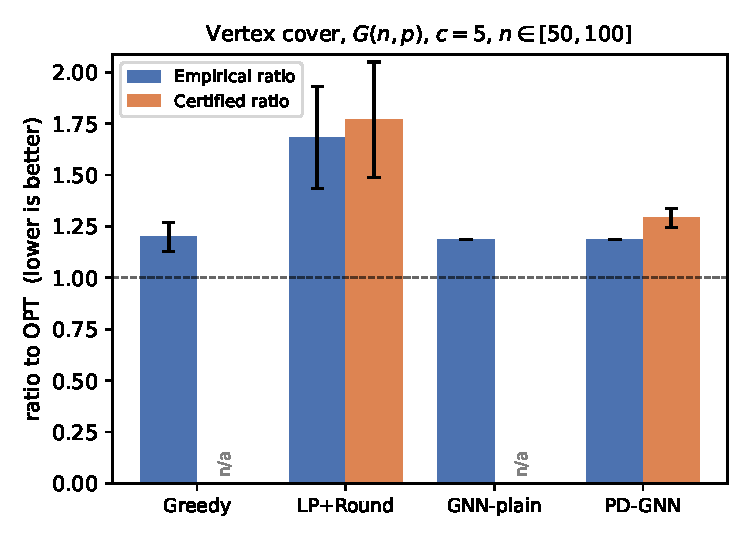
\includegraphics[width=0.48\linewidth]{figures/ratios_er5.pdf}\hfill
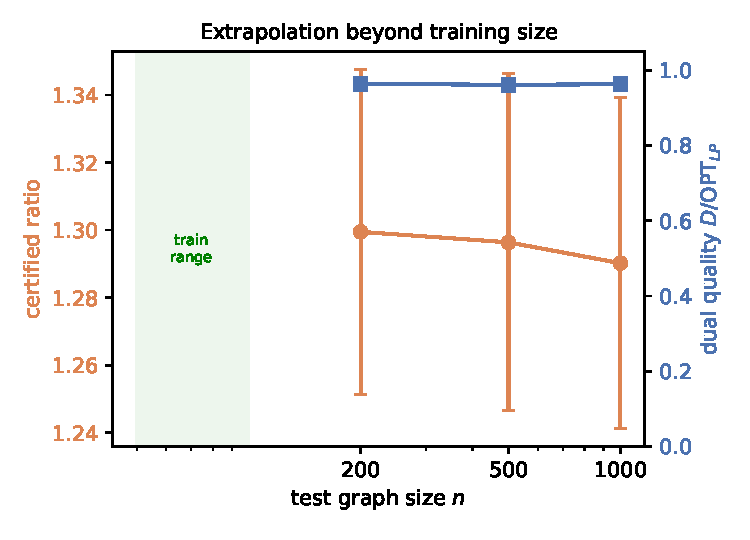
\includegraphics[width=0.48\linewidth]{figures/extrapolation.pdf}
\caption{Left: empirical and certified ratios on $G(n,p)$, $c=5$ (Table~\ref{tab:main}); the certified bar appears only for the two methods that emit a dual. Right: the \PDGNN{} certified ratio and dual quality as the test size grows past the training range.}\label{fig:res}
\end{figure}

\paragraph{Summary.} The experiments confirm the paper's actual claim (Theorem~\ref{thm:cert}): a learned network can emit an always-valid, instance-specific certificate, and with training that certificate is tight. They also surface an honest limitation of the objective rather than the architecture, which Section~\ref{sec:conc} takes up.


\section{Conclusion and Limitations}\label{sec:conc}
We argued that a learned combinatorial optimizer should report not just a
solution but a proof of its quality, and that the cleanest way to get such a
proof is to align the architecture with the primal--dual schema rather than to
read a certificate off a loss. \PDGNN{} carries coupled primal and dual states,
enforces both kinds of feasibility by construction, and so emits a certificate
that is always valid (Theorem~\ref{thm:cert}). Under the alignment condition of
Definition~\ref{def:align} its sample complexity is set by the round count of the
imitated scheme and the maximum degree rather than the number of nodes
(Theorem~\ref{thm:gen} and Corollary~\ref{cor:size}).

\paragraph{Limitations.}
Several caveats qualify these claims. The message-passing substrate is limited by
the Weisfeiler--Leman hierarchy, so \PDGNN{} cannot tell apart instances that are
WL-indistinguishable, and any problem whose primal--dual template needs such
distinctions is out of reach without higher-order features. The tightness of the
certificate, though never its validity, is fundamentally limited by the
integrality gap of the relaxation: the tightest certificate any model can report
is $\OPT/\OPTLP$, so on instances with a large gap even a perfect dual head gives
a loose though valid bound. For set cover the gap is $\Theta(\log n)$, which caps
the certificate at $O(\log n)$. Empirically (Section~\ref{sec:exp}) we found a
sharper limitation that lies in the \emph{objective} rather than the
architecture: the size-normalized loss \eqref{eq:loss} rewards a large dual but
places no reward on the primal scores, so $\mu^{(T)}$ collapses toward zero and
the integral cover is produced entirely by the repair layer. The dual head still
learns a near-LP-optimal feasible dual, so the certificate is meaningful, but the
\emph{learned} content of the cover is lost. A natural fix is to add a primal
term that rewards complementary-slackness-consistent coverage---for instance a
hinge on $\sum_{(u,v)}\mathrm{ReLU}(1-\mu_u-\mu_v)$ or a supervised primal target
on small instances---so that the learned primal is no longer vacuous; we leave a
careful study of this to future work. The generalization bound carries the usual
factor exponential in $T$, which is probably loose, and tightening it with
algorithm-specific stability arguments instead of generic covering numbers is the
main open question. Finally, going beyond covering LPs---to packing problems, to
problems with exponentially many constraints handled by separation oracles, and
to dualities that are not LP-based---would show how far the
architecture-as-algorithm idea reaches.

\bibliographystyle{plainnat}
\bibliography{refs}

\end{document}
